\documentclass{beamer}
\usepackage{ctex, hyperref}
\usepackage[T1]{fontenc}
\usepackage{bookmark}
\usepackage{amsmath}
\usepackage{latexsym,amsmath,xcolor,multicol,booktabs,calligra}
\usepackage{graphicx,pstricks,listings,stackengine,subfigure,extpfeil}
\usepackage{wrapfig}
\author{Wangxianyi}
\usepackage{graphicx}
\usepackage{algorithm}
\usepackage{algpseudocode}
\usepackage{multirow}
\title{MAPDP: \newline Cooperative Multi-Agent Reinforcement Learning to Solve Pickup and
Delivery Problems}
\institute{LZU}
\date{\today}

\usepackage{NJUPT}

\def\cmd#1{\texttt{\color{red}\footnotesize $\backslash$#1}}
\def\env#1{\texttt{\color{blue}\footnotesize #1}}
\definecolor{deepblue}{rgb}{0,0,0.5}
\definecolor{deepred}{rgb}{0.6,0,0}
\definecolor{deepgreen}{rgb}{0,0.5,0}
\definecolor{halfgray}{gray}{0.55}

\lstset{
    basicstyle=\ttfamily\small,                                                                                                                                                                                                                                           
    keywordstyle=\bfseries\color{deepblue},
    emphstyle=\ttfamily\color{deepred},    % Custom highlighting style
    stringstyle=\color{deepgreen},
    numbers=left,
    numberstyle=\small\color{halfgray},
    rulesepcolor=\color{red!20!green!20!blue!20},
    frame=shadowbox,
}

\begin{document}

\kaishu
\begin{frame}
	\titlepage
\end{frame}

\begin{frame}
	\tableofcontents[sectionstyle=show,subsectionstyle=show/shaded/hide,subsubsectionstyle=show/shaded/hide]
\end{frame}


\section{Introduction}

\begin{frame}{Background Introduction}
	\begin{itemize}
		\item Vehicle Routing Problem (VRP) is crucial in various real-world applications such as express systems, industrial warehousing, and on-demand delivery.
		\item Cooperative Pickup and Delivery Problem (PDP) is a variant of VRP that plays a significant role in applications like on-demand delivery and industrial logistics.
		\item Challenges in solving cooperative PDP include structural dependency between pickup and delivery pairs and the need for effective cooperation among different vehicles.
		\item Existing solutions face difficulties in explicit modeling of dependencies and cooperation, leading to suboptimal performance.
	\end{itemize}
\end{frame}

\begin{frame}{Research Objectives}
	\begin{itemize}
		\item Explore the cooperative Pickup and Delivery Problem (PDP) with multiple vehicle agents using Multi-Agent Reinforcement Learning (MARL).
		\item Design a centralized MARL framework to generate cooperative decisions by capturing the inter-dependency of heterogeneous nodes.
		\item Train different agents based on communication embedding using a specially designed cooperative Advantage Actor-Critic (A2C) algorithm.
		\item Evaluate the effectiveness of the MAPDP framework on different datasets and compare its performance with existing baselines.
	\end{itemize}
\end{frame}

\begin{frame}{Overview of MAPDP Framework}
	\begin{itemize}
		\item MAPDP is a novel cooperative Multi-Agent Reinforcement Learning (MARL) framework designed to solve the Cooperative Pickup and Delivery Problem (PDP).
		\item The framework utilizes multi-agent cooperation to generate high-quality solutions by sharing a common context encoder and individual decoders for each vehicle agent.
		\item MAPDP learns to generate the next node to visit for each vehicle agent step by step and outputs a complete routing plan.
		\item Key components of MAPDP include paired context embedding to represent node dependencies, cooperative decoders for decision dependence, and a cooperative A2C algorithm for model training.
	\end{itemize}
\end{frame}

\section{Problem Formulation}

% \begin{frame}{Introduction to Cooperative Pickup and Delivery Problem (PDP)}
% 	\begin{itemize}
% 		\item Node Representation
% 		\item Node Pairing
% 		\item Spatial Distances
% 		\item Demand Volume
% 		\item Assignment to Vehicles
% 		\item Routing Decision
% 		\item Arrival Time
% 		\item Routing Sequence
% 	\end{itemize}
% \end{frame}

\begin{frame}{Mathematical Modeling of Cooperative PDP}
	\centering

	% \mathrm{Let}x_{ijk}\in\{0,1\}\mathrm{denote}\mathrm{whether}\mathrm{the}\mathrm{vehicle}k\mathrm{travels}\\\mathrm{directly~from~node~}v_i\mathrm{~to~node~}v_i,\mathrm{~and~}T_i\mathrm{~as~the~arrival~time}
	\begin{align}
		\mathrm{min} \sum_{k=1}^{K}\sum_{i=0}^{2N}\sum_{j=1}^{2N+1}e_{ij}x_{ijk}
	\end{align}
	\begin{itemize}
		\small
		\item $x_{ijk}\in\{0,1\}$: whether the vehicle $k$ travels directly from node $v_i$ to node $v_j$.
		\item $e_{ij}$: spatial distances.
	\end{itemize}
	\begin{align}
		\sum_{k=1}^{K}\sum_{j=1}^{2N+1}x_{ijk}=1,\forall i\in[0,2N]
	\end{align}

	\begin{align}
		\sum_{k=1}^{K}\sum_{i=0}^{2N}x_{ijk}=1,\forall j\in[1,2N+1]
	\end{align}
\end{frame}

\begin{frame}{Mathematical Modeling of Cooperative PDP}
	\begin{align}
		\sum_{i\in S^{\prime}}d_{i}\leq C_{k},\forall S^{\prime}\subseteq S,\forall k\in[1,K]
	\end{align}
	\begin{itemize}
		\small
		\item $d_i$: Each pickup order has a demand volume.
		\item $C_k$: Capacity of the k-th vehicle.
		\item $S$: A consecutive routing sequence from $v_0$ and ends at $v_{2N+1}$.
	\end{itemize}
	\begin{align}
		\sum_{j=1}^{2N+1}x_{i,jk}=\sum_{j=0}^{2N+1}x_{i+N,jk},\forall k\in[1,K],i\in[1,N]
	\end{align}
	\begin{align}
		T_{i}\leq T_{i+N},\forall i\in[1,N]
	\end{align}

\end{frame}

\section{Methodology}


\begin{frame}{Explanation of State, Action}
	\begin{columns}
		\begin{column}{0.4\textwidth}
			\begin{itemize}
				\small
				\item State: At step $t$, agent $k$'s state includes its remaining capacity $C_k^t$ and current trajectory $S_k^t$. The current location, the last visited node, is denoted by $v_{I_k^t}$, where $I_k^t$ is the node index. All vehicles can communicate centrally, ensuring full observability in the cooperative PDP setting.
				\item Action: The action at step $t$ for vehicle agent $k$ is to determine a node as its next target, represented as $v(k,t).$
			\end{itemize}
		\end{column}
		\begin{column}{0.6\textwidth}
			\centering
			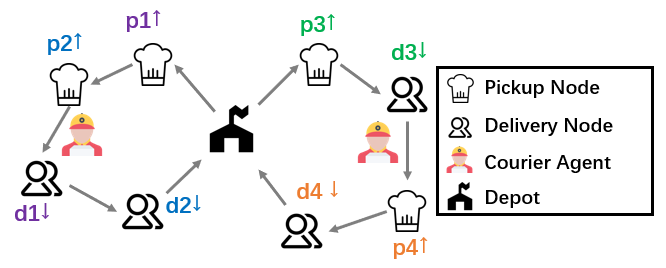
\includegraphics[width=\textwidth]{show.png} % 用正确的图像文件名替换 your_image.jpg
		\end{column}
	\end{columns}
\end{frame}


\begin{frame}{Explanation of Transition, Reward}
	\begin{columns}
		\begin{column}{0.4\textwidth}
			\tiny
			\begin{itemize}
				\item Transition: The transition between adjacent states is to replace every agent to its target node as its current action. Then we update both the trajectory and the remaining capacity of each agent: $S_k^{t+1}=(S_k^t;\{v_{I_k^t}\}), C_k^{t+1}=C_k^t-d_{I_k^t}$, where ; means concatenating the partial solution with the new selected node.
				\item Reward: All agents aim to minimize the total travel distance during the episode. At each step, the reward $r_k^t$ is the negative length of the newly traveled arc, and the final episode reward $R$ is the sum of all individual rewards $r_k^t$, where $T$ is the total number of decision steps in an episode, and $I_k^0=0$ denotes that all vehicles start from depot $v_0$.
			\end{itemize}
		\end{column}
		\begin{column}{0.6\textwidth}
			\centering
			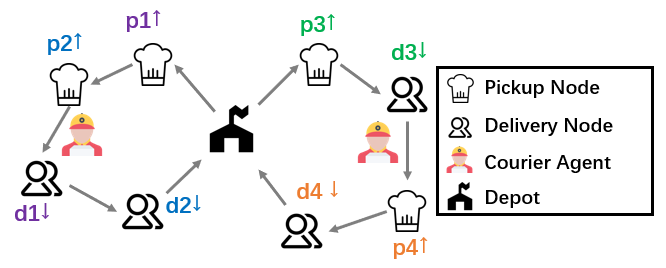
\includegraphics[width=\textwidth]{show.png} % 用正确的图像文件名替换 your_image.jpg
		\end{column}
	\end{columns}
\end{frame}

\section{MAPDP}

\begin{frame}{Overview of MAPDP Framework}
	\begin{figure}
		\centering
		\hspace{-1.2cm} % Adjust the value to move the image to the left
		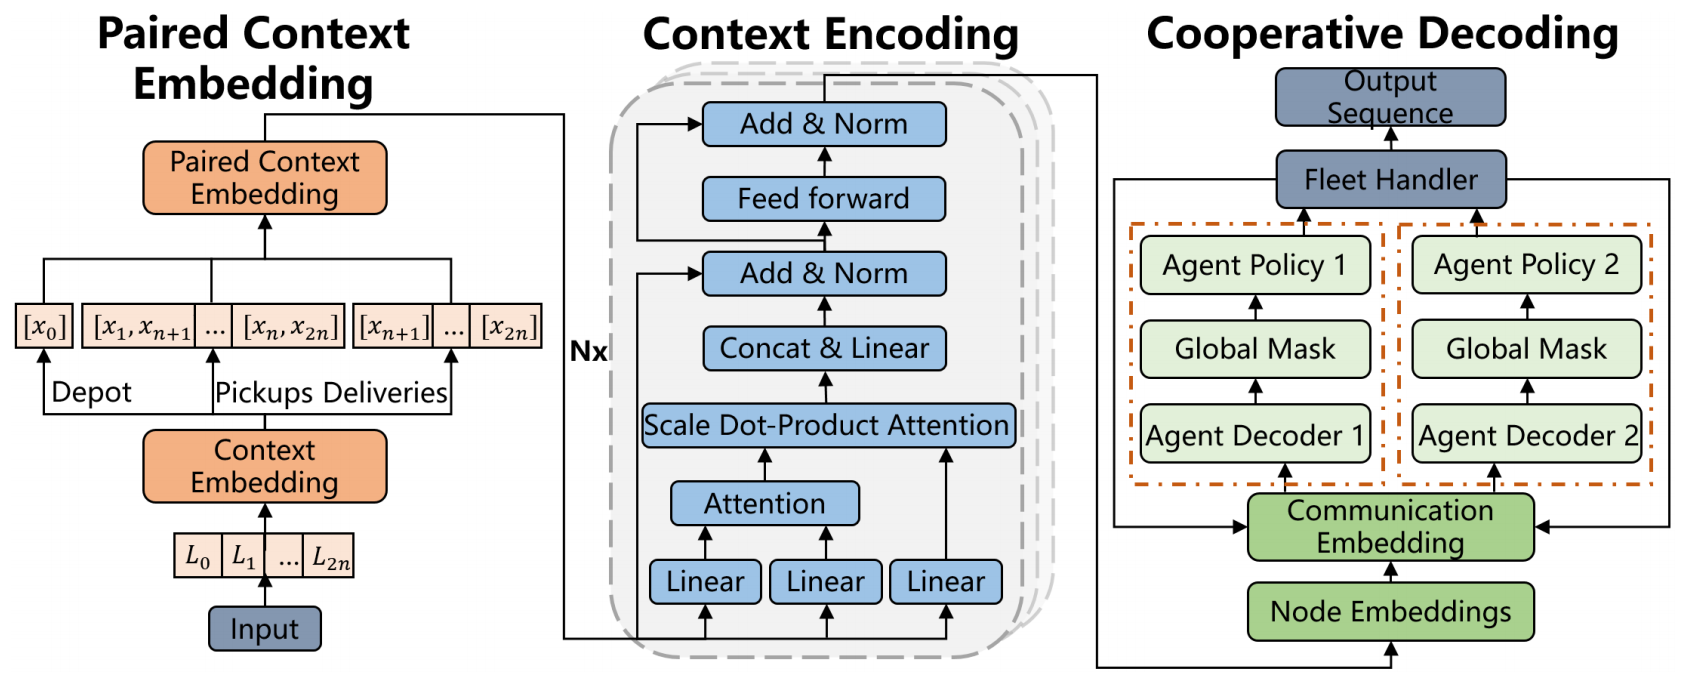
\includegraphics[scale=0.199]{model_structure.png}
		\caption{MAPDP Framework}
	\end{figure}
\end{frame}

\begin{frame}{Paired Context Embedding}
	Original 2-D location information : $\mathcal{L}_{i}$ \\
	Concatenat the two features and map them into one dense vector : $x_{i}=W^{x}[\mathcal{L}_{i},d_{i}]+b^{x}.$\\

\end{frame}

\begin{frame}{Paired Context Embedding}
	\begin{columns}
		\begin{column}{0.6\textwidth}
			\footnotesize
			\begin{align}
				h_i^0=\begin{cases}W_0^xx_i+b_0^x,&i=0,\\W_p^x[x_i;x_{i+N}]+b_p^x,&1\le i\le N,\\W_d^xx_i+b_d^x,&N+1\le i\le2N,\end{cases}
			\end{align}

			\begin{align}
				\hat{h_{i}}=BN^{\ell}(h_{i}^{\ell-1}+MHA_{i}^{\ell}(h_{1}^{\ell-1},h_{2}^{\ell-1},\cdots h_{2N}^{\ell-1})),
			\end{align}

			\begin{align}
				h_{i}^{\ell}=BN^{\ell}(\hat{h_{i}}+FF^{\ell}(\hat{h_{i}})).
			\end{align}
		\end{column}
		\begin{column}{0.4\textwidth}
			\centering
			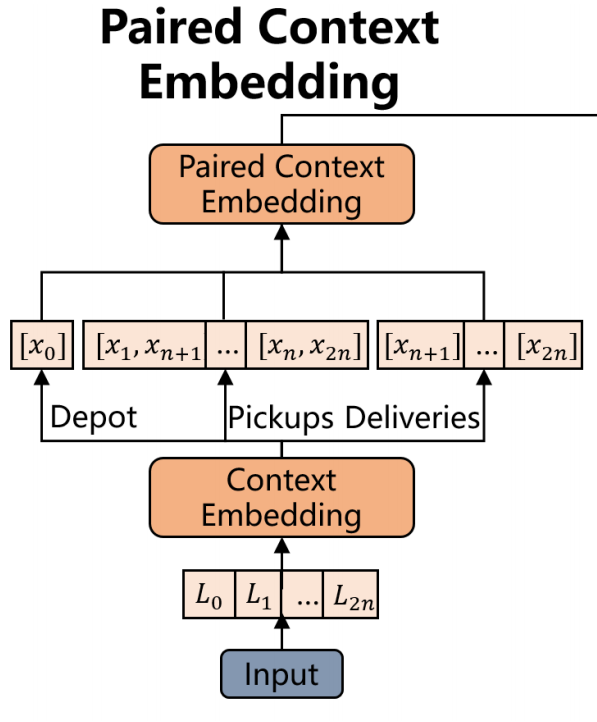
\includegraphics[width=\textwidth]{PCE.png} % 用正确的图像文件名替换 your_image.jpg
		\end{column}
	\end{columns}
\end{frame}


\begin{frame}{Context Encoding}
	\begin{columns}
		\begin{column}{0.6\textwidth}
			\footnotesize
			\begin{align}
				Q_i^h,K_i^h,V_i^h=W_Q^hh_i,W_K^hh_i,W_V^hh_i,
			\end{align}

			\begin{align}
				A_i^h=softmax(Q_i^h{K^h}^T/\sqrt{d_k})V_j^h,
			\end{align}

			\begin{align}
				MHA_i=Concat(A_i^1,A_i^2,...,A_i^H)W_O,
			\end{align}
		\end{column}
		\begin{column}{0.4\textwidth}
			\centering
			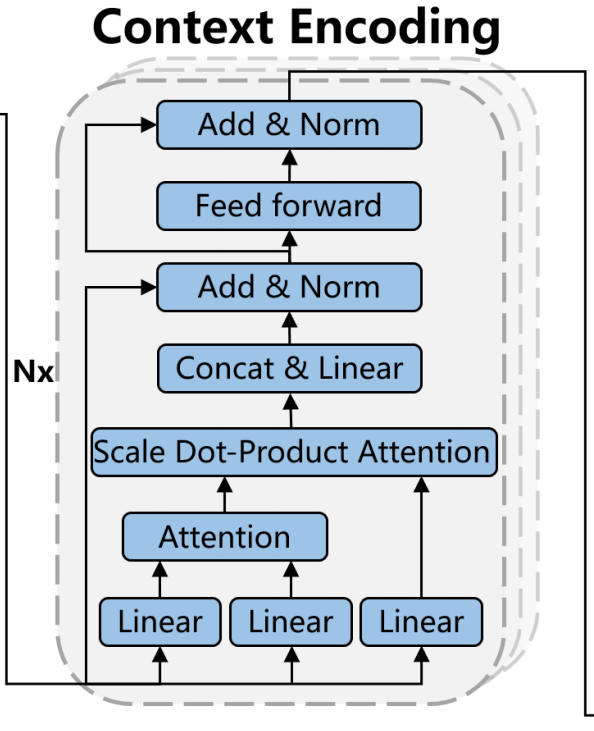
\includegraphics[width=\textwidth]{CE.png} % 用正确的图像文件名替换 your_image.jpg
		\end{column}
	\end{columns}

\end{frame}

\begin{frame}{Cooperative Multi-Agent Decoders}
	\begin{columns}
		\begin{column}{0.6\textwidth}
			\footnotesize
			\begin{align}
				Comm^t=[h_{I_1^t};C_1^t;h_{I_2^t};C_2^t;...;h_{I_K^t};C_K^t]
			\end{align}

			\begin{align}
				g_{k}^{t}=MHA_{k,(c)}(h_{1},h_{2},...,h_{2N}),
			\end{align}

			\begin{align}
				Q_{k}^{t},K_{k,i}^{t}=W_{Q,k}g_{k}^{t},W_{K,k}h_{i},
			\end{align}

			\begin{align}
				u_{k,i}^{t}=Dtanh(Q_{k}^{t}{}^{T}K_{k,i}^{t}/\sqrt{d_{k}}),
			\end{align}

			\begin{align}
				p_{\theta_{k},\phi}(v(k,t))=softmax(Mask^{t}(u_{k,i}^{t})),
			\end{align}
		\end{column}
		\begin{column}{0.4\textwidth}
			\centering
			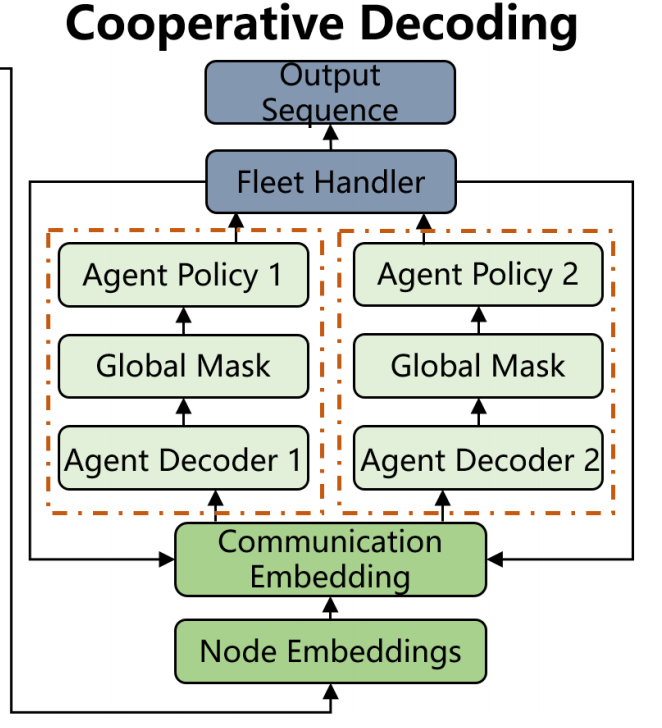
\includegraphics[width=\textwidth]{CD.png} % 用正确的图像文件名替换 your_image.jpg
		\end{column}
	\end{columns}
\end{frame}

\section{Experiments}

\begin{frame}{Evaluation Results on Different Datasets}
	\begin{figure}
		\centering
		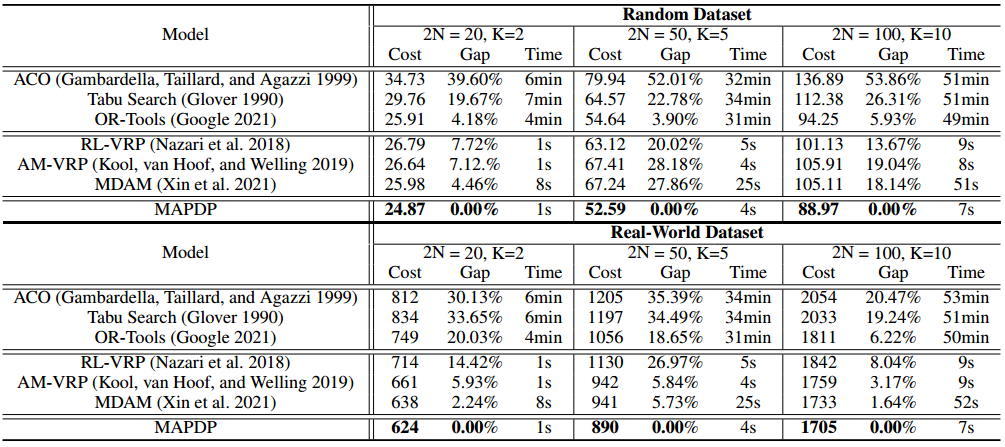
\includegraphics[scale=0.3]{table1.png}
		\caption{Comparison of Different Models on Random and Real-World Datasets}
	\end{figure}
\end{frame}

\begin{frame}{Performance Comparison with Other Methods}
	\begin{figure}
		\centering
		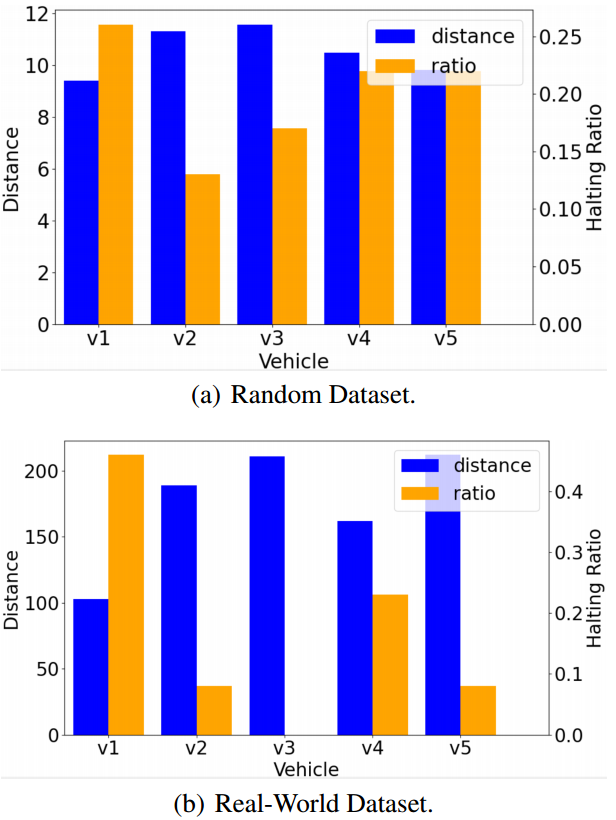
\includegraphics[scale=0.2]{graph.png}
		\caption{ Case studies on vehicle cooperation analysis from two datasets.}
	\end{figure}
\end{frame}

\section{Conclusion}

\begin{frame}{Conclusion}
	\begin{itemize}
		\item The proposed MAPDP framework leverages Multi-Agent Reinforcement Learning (MARL) to effectively solve the Cooperative Pickup and Delivery Problem (PDP) by capturing dependencies and promoting cooperation among multiple vehicles.
		\item MAPDP outperforms existing baselines by at least 1.64% in all experiment settings, demonstrating its superior performance in generating high-quality solutions for PDP.
		\item The centralized MARL framework, paired context embedding, cooperative decoders, and cooperative A2C algorithm collectively contribute to the success of MAPDP in addressing the challenges of PDP.
		\item Future research directions may include exploring scalability of MAPDP to larger problem instances, incorporating real-time constraints, and adapting the framework to dynamic environments.
	\end{itemize}
\end{frame}

\section{References}

\begin{frame}[allowframebreaks]
	\bibliography{ref}
	\bibliographystyle{njupt}
\end{frame}

\begin{frame}
	\begin{center}
		{\Huge \calligra Thanks!}
	\end{center}
\end{frame}

\end{document}